%%%%%%%%%%%%%%%%%%%%%%%%%%%%%%%%%%%%%%%%%%%%%%%%%%%%%%%%%%%%%%%%%%%%%%%%%%%%%%%%
%2345678901234567890123456789012345678901234567890123456789012345678901234567890
%        1         2         3         4         5         6         7         8

\documentclass[letterpaper, 10 pt, conference]{ieeeconf}  % Comment this line out if you need a4paper

%\documentclass[a4paper, 10pt, conference]{ieeeconf}      % Use this line for a4 paper

\IEEEoverridecommandlockouts                              % This command is only needed if
                                                          % you want to use the \thanks command

\overrideIEEEmargins                                      % Needed to meet printer requirements.

% See the \addtolength command later in the file to balance the column lengths
% on the last page of the document

% The following packages can be found on http:\\www.ctan.org
%\usepackage{graphics} % for pdf, bitmapped graphics files
%\usepackage{epsfig} % for postscript graphics files
%\usepackage{mathptmx} % assumes new font selection scheme installed
%\usepackage{times} % assumes new font selection scheme installed
%\usepackage{amsmath} % assumes amsmath package installed
%\usepackage{amssymb}  % assumes amsmath package installed

\usepackage{graphicx}
\usepackage{epsfig} % less modern
\usepackage{amsmath}
\usepackage{amssymb}
\usepackage{multirow}
\usepackage{subfigure}
\usepackage{graphicx,epstopdf}
\def\degree{${}^{\circ}$}
	
\title{\LARGE \bf
RRT-GD: An Efficient Rapidly-exploring Random Tree Approach with Goal Directionality for Redundant Manipulator Path Planning
}


\author{Junxiang Ge$^{1}$, Fuchun Sun$^{1}$, Chunfang Liu$^{1}$% <-this % stops a space
%\thanks{*This work was not supported by any organization}% <-this % stops a space
\thanks{$^{1}$State Key Lab of Intelligent Technology and Systems, Tsinghua National Laboratory for Information Science and Technology (TNList), Department of Computer Science and Technology, Tsinghua University. {\tt\small gejx14@mails.tsinghua.edu.cn, fcsun@tsinghua.edu.cn, cfliu1985@gmail.com}}%
}

\begin{document}



\maketitle
\thispagestyle{empty}
\pagestyle{empty}


%%%%%%%%%%%%%%%%%%%%%%%%%%%%%%%%%%%%%%%%%%%%%%%%%%%%%%%%%%%%%%%%%%%%%%%%%%%%%%%%
\begin{abstract}
Rapidly-exploring random trees (RRT) method performs well for obstacle-avoiding motion planning. However, it is not fast enough and less goal-direction. In this paper, we propose an effective rapidly-exploring random trees method with goal directionality (RRT-GD)  for redundant manipulator path planning. The presented RRT-GD model concentrates both on the status of the end actuator and on the movements of the joints that the Newton-Raphson method is employed for inverse kinematics calculation. In order to speed up the path planning, the path searching algorithm is modified to be goal-directionality and the quintic polynomial is applied to smooth the planned path. In the experiments, it shows that RRT-GD tends to be 10 or more times faster than the usual RRT algorithm when doing the same obstacle-avoiding path planning task. Therefore, RRT-GD could be more efficient and useful in doing our daily works.
\end{abstract}


%%%%%%%%%%%%%%%%%%%%%%%%%%%%%%%%%%%%%%%%%%%%%%%%%%%%%%%%%%%%%%%%%%%%%%%%%%%%%%%%
\section{Introduction}
 Rapidly-exploring random trees (RRT) method was proposed by SM Lavalle and JJ Kuffner [1], which is a suitable way to be used in obstacle-avoiding path planning for mobile robot or multiple freedom manipulator. It constructs a graph with obstacle free points in feasible space based on random sampling, in which the optimal path is searched from the initial point to the goal point.
 RRT method has the following superior characteristics comparing with other obstacle-avoiding methods:

\begin{itemize}
\item RRT method attends to explore unknown space.
\item The graph constructed by RRT will gradually fill up the feasible space if the exploring times is enough.
\item RRT method don't need precise modeling of the obstacles, instead, it only needs the information if or not a point is obstacle free through doing collision detect, thus ending up with the high efficiency of obstacle free planning.
\end{itemize}

Though it has the above advantages, RRT method will still perform low success rate of planning when there is many obstacles surrounded, or the distance from the initial point to the goal point is very far to explore. For these problems, JJ Kuffner and SM Lavalle [2, 3] proposed a bi-directional RRT algorithm (bi-RRT) that two trees were built based on the initial point and the goal point separately. When expanding each time, the tree of initial point will extend to the goal-point based tree, or the contrary way, until these two trees meets. Because of goal heuristic, this approach improves the success rate of path planning. In spite of this modification, we still find it defective sometimes for path planning.

As mentioned before, RRT attends to explore unknown space, so that it could explore the whole free space. However, for goal-reaching works, it does not need to explore the whole space in the most time. What we need to do is to find a feasible way from the initial point to the goal point without obstacle collision, i.e., only a part of the whole space is necessary for exploration, which includes the initial point, the goal point and some obstacles. Thus, in this paper, we propose a modified RRT method with goal directionality (RRT-GD) for path planning with goal-directionality exploration. The experiments demonstrate that the proposed method could quickly accomplish the obstacle avoiding path planning and the planning speed is 10 times faster than that of the original RRT method.

On the other hand, for performing the redundant manipulator motion, it is necessary to transform each point in the path tree from the configuration space (C-space) to robots' joint space by using the inverse kinematics optimization. There are lots of methods to do inverse kinematics optimization for redundant manipulator, e.g., MLG (most likeyly gradient method) [4, 5], WLN (weighted least norm method) [6], Genetic Algorithm [7], GP (gradient projection method), etc. In this paper, Newton-Raphson method is adopted to perform the inverse kinematics optimization work. In order to make comparation, we also implement MLG method in our exprements according to [4, 5].
Compared to other methods, Newton-Raphson method has faster converging speed and more accurate result that it takes less than 10 iteration times (usually 5 or 6 times) and has deviations less than mocro-meters. Finally, the quintic polynomial approach [8] is utilized to smooth the path from the initial point to the goal point with detailed status information (pose \& joint angles).

The paper is organized as follows. In Section II, the proposed RRT-GD approach is illustrated in detail; Section III introduce the Newton-Raphson method in inverse kinematics optimization; then, the quintic polynomial method is showed for smoothing path; in the section IV, we demonstrate the experiments for verifying the effectiveness of the proposed method.

\section{RRT with Extended Steps}

In this section, the original RRT method for obstacle-avoiding path planning is introduced firstly. Then, we show the presented RRT-GD approach for faster motion planning with goal directionality.

\subsection{Rapidly-exploring Random Trees}

The basic problem of RRT is how could we move the manipulator from the initial status to the goal status without collision with the obstacles in the space? To make it more clearly, we make appointments on the following mathematical symbols to express status space (S-space) and configuration space (C-space).

We use $n$ to stand for the degree of freedom (DOF) of the robot manipulator, which is 7 in our exprement. So S-space is expressed with 7 parameters from $q_1$ to $q_7$, with the expression like (1):

$$
S \ = \ (q_{1}, q_{2}, \ ...  \ , q_{7}) \eqno({1})
$$

As for the C-space, i.e., pose space, we use Euler angles that obeys Euler Z-X-Z transformation rules to express the azimuth angles, which displays like $\gamma = (\psi, \theta, \phi)$. Position writes like $P=(x,y,z)$. Get the position and Euler angles together, we define $m$ as the dimension of pose, which is 6 in this way, and the expression of pose is expressed like (2):

$$
X = (P,\gamma) = (x,y,z,\psi,\theta,\phi) \eqno({2})
$$

Note that $n > m$ should be guatanteed since it is a redundant system. Therefore, we get the initial condition of collsion-free path planning problem as this: knowing the initial joints' angle $S_{0}\in \mathbb{R}^n$, the initial status of the end-effector $X_{0}\in \mathbb{R}^m$ (which could be computed from $S_{0}$), and the goal status of the end-effector $X_{g}\in \mathbb{R}^m$. The relevant notations and functions of RRT are illustrated as below:

\begin{itemize}

\item $A_{0}$: the whole pose space which can be reached by robot manipulator in C-space. 

\item $A_{free}$: free space belong to $A_{0}$, i.e., $A_{free} \in A_{0}$, and there is no obstacle in $A_{free}$.

\item $A_{obs}$: space of obstacle, i.e., $A_{obs} = A_{0}  \backslash A_{free}$.

\item $B_{0}, B_{free}, B_{obs}$: these are the corresponding notations with A, but in the S-space. The subscripts take same meanings as in A.

\end{itemize}

Actually, it is difficult to build the accurate boundary of $A_{0}$. In convenient, we use $X_{min}$ and $X_{max}$ as the two terminal vertex of $A_{0}$ here.

\begin{equation}
A_{0} = \{X|\ X_{min} < X < X_{max}\}.
\label{eq_a0}
\end{equation}

RRT method builds a path tree $T = (V, E)$, with the initial point $X_{0}$ for pose and $S_{0}$ for status as the first tree point, while $V$ stands for all points and $E$ is the relation between these points (father point and its child). The basic functions that RRT method use are defined as follow:

\begin{itemize}

\item \textit{sample}:  generate a random point $X_{ram}$ in pose format within $A_{free}$.

\item \textit{distance}:  compute the distance between two points in $A_{0}$ by using (\ref{rrtDistance}).

\item \textit{nearest\_neighbor}: given the point X, this function returns the nearest point $X_{near}$ to X in $T$.

\item \textit{steer}: given the random point $X_{ram}$ and $X_{near}$, this function returns a new point $X_{new}$ in $A_{free}$, which is nearer to $X_{ram}$ than $X_{near}$.

\item \textit{collisionTest}: given point $X$, return 1 for obstacle free and 0 for obstacle collision.

\end{itemize}

Then, the basic algorithm of RRT is displayed as the pseudocode in Fig. \ref{fig_rrt}.

\begin{figure}[thpb]
      \centering
      \framebox{
      \parbox{3in}
      {
      $
      RRT (S_{0}, A_{0})\\
      1.\ V \leftarrow \{S_{0}\}; E \leftarrow \o; i \leftarrow 0;\\
      2.\ while\ i < N\ do \\
      3.\ \{ \\
      4.\qquad T \leftarrow (V,\ E); \\
      5.\qquad X_{rand} \leftarrow sample(i); i \leftarrow i+1; \\
      6.\qquad T \leftarrow extend(T, X_{rand});\\
      7.\ \} \\
      $
      \\
      $
      extend(T, X_{rand}) \\
      1.\ X_{near}=  nearest\_neighbor(T, X_{rand});\\
      2.\ X_{new} = steer(X_{near}, X_{rand});\\
      3.\ if\ X_{new}\ and\ collisionTest(X_{new})\\\
      4.\qquad V \leftarrow V \cup \{X_{new}\};\\
      5.\qquad E \leftarrow E \cup \{(X_{near}, X_{new})\};\\
      5.\qquad return\ success;\\
      6.\ else\\
      7.\qquad return\ fail;
      $
	 }
}
      \caption{The pseudocode of RRT algorithm.}
      \label{fig_rrt}
\end{figure}

In our algorithm, a `rrtDistance' is employed for calculating the distance between points as (\ref{eq_rrtDistance}). It is made to concentrate more on the accuracy of position than the accuracy of Euler azimuth angles.

 \begin{equation}
 \begin{array}{ll}
 &rrtDistance(X_{1},X_{2})=\alpha ||P_{1}-P_{2}|| + \\
& \qquad\qquad (1-\alpha) ||\gamma_{1}-\gamma_{2}||, \ 0 < \alpha < 1.
 \end{array}
 \label{eq_rrtDistance}
 \end{equation}

 In our exprements, we choose $\alpha > 0.5$, e.g., $\alpha = 0.8$. The \textit{sample} function generates a point $A_{0}$ that $X_{min} < A_{0} < X_{max}$. Then, the random point $X_{ram}$ is produced with the \textit{sample} function as shown in  (\ref{eq_sample}).

 \begin{equation}
 X_{ram} = X_{min} + t \times (X_{max}-X_{min}), 0<t<1;
  \label{eq_sample}
 \end{equation}

Notice that $t$ is randomly generated in the interval (0, 1) and the \textit{sample} function would produce all the points of $A_{0}$. As for the \textit{steer} function, a new point will be generated depending on $X_{near}$ and $X_{ram}$ as shown in (\ref{eq_ram}):

\begin{equation} \label{eq_ram}
 \begin{array}{rr}
 X_{new} = X_{near} + s(X_{ram}-X_{near})/||X_{ram}-&\\
 X_{near}||,\ 0<s<||X_{ram}-X_{near}||.&
 \end{array}
 \end{equation}

 We called $s$ in (\ref{eq_ram}) the step-length. In RRT algorithm, each time when \textit{steer} function runs, the RRT tree $T$ will attend to step $s$ length forward in $A_{0}$. Since $X_{rand}$ will be anywhere in $A_{0}$, it is inferred that the direction tree $T$ extends is all-dimension, i.e., no certain direction, but different directions with different times. These properties of RRT method will be discussed in the next subsection.

\subsection{Modified RRT Approach}

Though RRT can explore the whole space $A_{0}$ to get an obstacle-free path to reach the goal point, it still has some shortage when it actually runs. Since RRT extends only one step (with step-length $s$) further each time, it seems slow sometimes when $A_{0}$ is big enough to explore. On the other hand, RRT tree is built beginning with the initial point, leaving out the goal point in the tree-built process. Still, there are other insufficients with RRT, which results in many modified RRT methods. Bi-RRT [2, 3] is one of them. Here, we briefly introduce this modified model.

Bi-RRT extends more steps until the new point generated  is in collision with obstacles or reach the random point $X_{ram}$. And bi-RRT maintains two trees in its memory, one starting extend function from the initial point and the other from the goal point. The two trees extend to each other interchangeably every time until they meet in the space, which is the reason the name `bi-RRT' comes from. With such modification, bi-RRT takes in account of both the initial point and the goal point together with a faster extending speed. Nevertheless, it still has not solve the problem of exploring unuseful space since the two trees will both explore the whole space.

In our model, multiple steps extending strategy is integrated into our algorithm. The multi-extend algorithm is written as shown in Fig. \ref{fig_multiExtend}:

\begin{figure}[thpb]
      \centering
      \framebox{
      \parbox{3in}
      {
      $
      multi\_extend(T, X_{rand})\\
      1.\ [X_{new}, result] = extend(T, X_{rand});\\
      2.\ if\ result = fail\ or\ collisionTest(X_{new}) = 0\\
      3.\qquad return\ fail;\\
      4.\ while\ result = success \\
      5.\ \{ \\
      6.\qquad [X_{new}, result] = extend(X_{new}, X_{rand});\\
      \begin{aligned}
      7.\qquad if\ collision&Test(X_{new}) = 0\ or\ \\ &surpass(X_{new}, X_{rand})\\
      \end{aligned} \\
      8.\qquad \qquad break; \\
      9.\ \} \\
      10.\ return\ success.
      $
	 }
}
      \caption{Multi-step extended pseudocode}
      \label{fig_multiExtend}
\end{figure}

The function `$surpass(X_{new},X_{rand})$' detects if $X_{new}$ is near enough to $X_{rand}$. If the two points are close enough, then `true' returns and `multi\_extend' method will be stopped; Otherwise, the `false' returns and the extending process continues. It could be deduced that, if the extending direction is correct, i.e., closer to the goal point, we could reach the goal point faster; however, if extends to a bad direction frequently, this extending strategy will then take more time than one-step extending strategy. We solve this problem by presenting a RRT-GD (RRT with goal-directionality) model. 

\subsection{RRT-GD: Trun RRT to be goal-directionality}

As mentioned before, both RRT and its modified methods (includeing bi-RRT) are easy to explore unuseful space which do not need in the daily tasks, i.e., it lacks goal-directionality. In order to solve this problem, taking the normal task in our experiment circumstance into account, we turn our sights to the `sample' function in RRT. Simple to find that if we just don't use a whole space `sample' method, but limit it to a useful space, we can decide the extending direction of RRT tree $T$, that is the kernel principle within our modified RRT method called RRT-GD.

Originally, `sample' method is random in the whole work space, thus its extending direction is all-around. The sketch map can be seen in Fig. \ref{fig_sketch}. When we use a space containing the goal point $X_{g}$, called sample space $A_{sam}$, which can simply be a sphere with $X_{g}$ centering (of course other shapes also works, e.g., cuboid), the extending direction can be limit to goal-direction, as Fig. \ref{fig_sketch} shows. It can be seen from the sketch map that, if the initial point is contained in sample space, i.e., $X_{0}\in A_{sam}$, then the extending direction could also be all-around just as usual RRT does, but since the probability of the goal-direction becomes larger than the other directions, the principle of RRT-GD could also work.

\begin{figure}[thpb]
      \centering
      \framebox{
      \parbox{3in}{
      \subfigure[Extend direction of RRT: all-direction.]
      {
      \label{subfig1_sketch}
      \includegraphics[width=8cm, height=4.2cm]{ext2whole.eps}	
      }
      \subfigure[Extend direction of RRT-GD: goal-direction.]
      {
      \label{subfig2_sketch}
      \includegraphics[width=8cm, height=4.2cm]{ext2sample.eps}	
      }
      }
      }
      \caption{Extend direction of RRT and RRT-GD. Pink cuboid is for the whole working space. Blue sphere is for sample space. }
      \label{fig_sketch}
\end{figure}

With this change, RRT-GD needs less extending times and the tree it build will go to the goal point rapidly. But on the other hand, it could also be easily seen that RRT-GD can't get answer if all the extending direction of it can't be explored further, e.g., a big obstacle object stands between the initial point and the goal point so that it resist all the extending directions RRT-GD could generate out. That is truly a problem in theory, but RRT-GD could work well in fact because of the following reasons:

\begin{itemize}

\item In fact, we could not get the accurate profile of the whole space $A_{0}$ and $A_{ram}$ most of the time, so the method of choosing a big range of $A_{0}$ to satisfied our tasks itself is a RRT-GD method. In this way, RRT-GD is in the same with RRT, hence it will be all-direction exploring method and get the correct answer just as RRT will.
\item  As mentioned above, RRT-GD could also be all-direction if the sample space if $A_{sam}$ include $X_{0}$. So RRT-GD could get the correct answer as RRT could.
\item In fact, there will not be so many obstacles, and each obstacle will not be so big in the working space for our common tasks. As long as we make $A_{sam}$ big enough, RRT-GD could always works correctly.  

\end{itemize} 

As we can see later in our exprements, RRT-GD could work faster and better than RRT most of time.

\section{Inverse Kinematics with Newton-Raphson method}

This section focuses on the inverse kinematics optimization for redundant manipulator. There has been some inverse kinematics methods, e.g., MLG (most likeyly gradient method) [4, 5], WLN (weighted least norm method) [6], Genetic Algorithm [7], GP (gradient projection method), etc.. Because of high accuracy and speed, we utilize the Newton-Raphson method to perform the inverse kinematics optimization task.


\subsection{Newton-Raphson method}

Let's come back to our inverse kinematics problem: we know $S_{0}$ (and so $X_{0}$ can be computed) and $X_{g}$, how could we compute $S_{g}$? Newton-Raphson method is an iteration approach that each time it just goes straight from the current point to the goal point.

\begin{equation}\label{Eq_NR}
S_{n+1} = S_{n} + J^{+} \times minus(X_{g}, X_{n}).
\end{equation}

The current status and pose are written as $S_{n}$ and $X_{n}$, and $J^{+}$ is the Jacobian matrix of current poin. Then when $X_{n}$ is close enough to $X_{g}$, we get the answer $S_{n+1}$ as result $S_{g}$. Note that though the function name called `minus', it didn't just do simple minus operation as `$X_{g} - X_{n}$', because the Euler azimuth doesn't supplement the minus operation. We should use the Rotate-By-1-Axis method to get the corret answer, since the combination of any fix-axis rotations of rigid body can be seen as one-time fix-axis rotation.

After this work, we take down the Newton-Raphson method as Fig. \ref{fig_newton}.

\begin{figure}[thpb]
      \centering
      \framebox{
      \parbox{3in}
      {
      $
      Newton\_Raphson(S_{0}, X_{g})\\
      1.\ compute\ X_{0}\ and\ J^{+}; i = 0; times = 0;\\
      2.\ while\ \epsilon < rrtDistance(X_{i}, X_{g})\ and\ times < N\\
      3.\ \{ \\
      4.\qquad S_{i+1} = S_{i} + J^{+}\times minus(X_{g}, X_{i});\\
      5.\qquad i = i + 1;times = times + 1;\\
      6.\qquad compute\ X_{i}\ and\ J^{+};\\
      7.\ \}
      $
	 }
}
      \caption{Newton-Raphson method pseudocode}
      \label{fig_newton}
\end{figure}

Here we use N (we set it to 10 in program) to limit the iteration times, for the fact that Newton-Raphson method would always get the correct answer in less than 10 iteration times with accuracy of micrometer, otherwise it would fail with bias greater than $\epsilon$ (1 micrometer), i.e., more iteration times have no use cause it can't improve the accuracy further more.

\subsection{Quintic Polynomial with Path Smoothing}

There comes another question after doing Newton-Raphson method: knowing $S_{0}$ and $S_{g}$, how could we move the manipulor? The most direct answer might be directly adapt the joint angles to $S_{g}$, however, it might not be the optimal path in the thought of end manipulator. Thus, we need to smooth the path from $S_{0}$ to $S_{g}$.

The quintic polynomial has been used in our program, the principle of which can be seen in [8]. We just use its conclusion. Supposed we know $S_{0}$, $S_{g}$, and their distance fixed, we need to plan the medium path in 1 second (of course it can be changed by timing a factor). Then in quintic polynomial method, we plan the path as in (\ref{eq_quintic}):

\begin{equation}
\begin{array}{c}
S(t) = a_{5}t^5+a_{4}t^4+a_{3}t^3+a_{2}t^2+a_{1}t+a_{0};\\
with:
\left \{
\begin{array}{ll}
a_{5} = &6(S_{g}-S_{0});\\
a_{4} = &-15(S_{g}-S_{0});\\
a_{3} = &10(S_{g}-S_{0});\\
a_{2} = &0;\\
a_{1} = &0;\\
a_{0} = &S_{0};\\
\end{array}
\right.
\end{array}
\label{eq_quintic}
\end{equation}

We can see in (\ref{eq_quintic}) of the kinematics properties of its planning path. When $t = 0s$, $S(t)$ equals to $S_{0}$, that is the initial point;  and when $t = 1s$, $S(t)$ equals to $S_{g}$, that is the goal point. And we can also compute the speed at each time in the path, just by doing differential operation. What we can deduce from (\ref{eq_quintic}) is that the speed of end manipulator when in initial point or goal point is 0. We could also change the coefficients from $a_{0}$ to $a_{5}$ according to [8] to fit different uses. These method works well on our 7-arm robot manipulator when doing exprements.

\section{Experiments}

\subsection{Experiment Environment}

We use a 7-DOF (degree of freedom) robot manipulator, show in Fig. \ref{robotGraph} to test the results in our experiment. Then we use the D-H method (Denavit and Hartenberg method) to model our robot arm, with the model axis built obeying D-H parameter method as the Fig. \ref{robotAxisGraph} show.

   \begin{figure}[thpb]
      \centering
      %\framebox{\parbox{2.2in}}
      \includegraphics{robotGraph.eps}
      \caption{7-DOF robot arm}
      \label{robotGraph}
   \end{figure}

   \begin{figure}[thpb]
      \centering
      %\framebox{\parbox{2.2in}}
      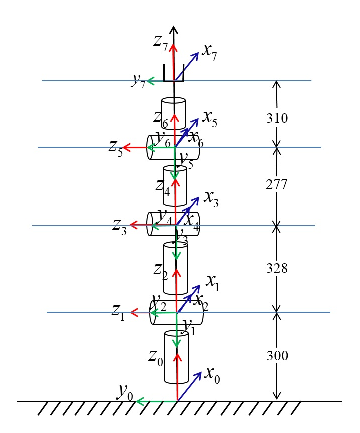
\includegraphics{robotaxis.eps}
      \caption{Robot axis coordinates, obeying D-H parameter method. Numbers in the graph is in milimeter.}
      \label{robotAxisGraph}
   \end{figure}

As a result of this axis coordinates, we get the DH parameters  (show in TABLE \ref{table1}) from it, which is the key data used in our procedure.

\begin{table}[h]
\caption{$DH\ Parameters\ of\ robot.\ (\theta: joint\ angle;\ d: connecting\ rod\ skew;\ a: connecting\ rod;\ \alpha: tortuosity\ angle\ of\ connecting\ rod.)$}
\label{table1}
\begin{center}
\begin{tabular}{c|ccccc}
\hline
Joint Number & $\theta_i$ & $d_i$(mm) & $a_i$(mm) & ${\alpha_i}$(\degree) & area of $\theta_i$(\degree) \\
\hline
1 & $q_1$ & 300 & 0 & -90 & -180$\sim$180\\
2 & $q_2$ & 0 & 0 & 90 & -90$\sim$90 \\
3 & $q_3$ & 328 & 0 & -90 & -180$\sim$180\\
4 & $q_4$ & 0 & 0 & 90 & -120$\sim$120\\
5 & $q_5$ & 277 & 0 & -90 & -180$\sim$180\\
6 & $q_6$ & 0 & 0 & 90 & -120$\sim$120\\
7 & $q_7$ & 310 & 0 & 0 & -180$\sim$180\\
\hline
\end{tabular}
\end{center}
\end{table}

\subsection{Comparation between Newton-Raphson and MLG}

At the beginning, we have complemented the MLG method before using Newton-Raphson method for inverse kinematics. Here, we introduce MLG method and compare it with Newton-Raphson method, to see the great properties of Newton-Raphson algorithm.

MLG method is also a iteration method, using the gradient of current point as the iteration direction, the detail of which can be seen in [4, 5]. We just make comparation between MLG and Newton-Raphson method.

\begin{table*}[h]
\caption{$Comparation\ between\ RRT\ and\ $ Newton-Raphson $ method.\ S_{0} = [0.7854;0.5236;0;0.5236;0;0.5236;0](rad);\ X_{0}=[0.5045;0.5045;0.7223;2.3562;1.5708;-1.5708];\ dist = rrtDistance(X_{0}, X_{g}), all\ their\ units\ are\ meters(m). `\surd'\ means\ successful.\ `\times'\ means\ result\ failed,\ i.e.,\ bias\ (accuracy)\ comes\ out\ more\ than\ 0.1m.$}
\label{table_newton}
\begin{center}
\begin{tabular}{c|c|c|c|c|c|c}
\hline
No. & task(m) & Method & iteration times & time spent($10^{-3}s$) & accuracy(m) & result \\
\hline
\multirow{4}{*}{1}  &
\multirow{4}{*}{
$
\begin{array}{l}
X_{g} =
\left[
\begin{array}{c}
0.50;
0.45;
0.72;
2.35;
1.57;
-1.57
\end{array}
\right] \\ \\
dist = 0.045.
\end{array}
$}
  & N-R & 5 & $6.15$ & $1.28\times 10^{-9}$ & $\surd$ \\
\cline{3-7}
  &    &         & 5 & $5.70$ & $6.50\times10^{-3}$ & $\surd$ \\ \cline{4-7}
   &    & MLG & 10 & $6.52$ & $2.64\times10^{-3}$ & $\surd$ \\ \cline{4-7}
   &    &         & 20 & $11.76$ & $1.25\times10^{-3}$ & $\surd$ \\
\hline
\multirow{4}{*}{2} &
\multirow{4}{*}{
$
\begin{array}{l}
X_{g} =
\left[
\begin{array}{c}
0.5;
0.48;
0.72;
2.35;
1.55;
-1.55
\end{array}
\right] \\ \\
dist = 0.025.
\end{array}
$
}
& N-R & 4 & 2.38 & $2.34\times10^{-7}$ & $\surd$ \\
\cline{3-7}
 &     &         & 5 & 3.95 & $9.74\times10^{-2}$ & $\surd$\\
\cline{4-7}
 &     &  MLG &10& 6.60 & $9.56\times10^{-2}$ & $\surd$\\
 \cline{4-7}
 &     &         &20& 12.77& $9.39\times10^{-2}$ & $\surd$\\
\hline
\multirow{4}{*}{3}
&
\multirow{4}{*}{
$
\begin{array}{l}
X_{g} =
\left[
\begin{array}{c}
0.44;
0.44;
0.68;
2.30;
1.57;
-1.57
\end{array}
\right] \\ \\
dist = 0.092.
\end{array}
$
}
& N-R & 7 &3.87 & $5.87\times10^{-8}$ & $\surd$ \\
\cline{3-7}
 &    &        & 5 & 3.94 & $1.65\times10^{-2}$ & $\surd$ \\
\cline{4-7}
 &    & MLG &10& 6.64 & $1.73\times10^{-2}$ & $\surd$ \\
 \cline{4-7}
 &    &         &20& 12.20& $1.78\times10^{-2}$ & $\surd$ \\
 \hline
\multirow{4}{*}{4}
&
\multirow{4}{*}{
$
\begin{array}{l}
X_{g} =
\left[
\begin{array}{c}
0.45;
0.55;
0.60;
2.00;
1.57;
-1.57
\end{array}
\right] \\ \\
dist = 0.184.
\end{array}
$
}
& N-R & 9 &5.70 & $5.53\times10^{-10}$ & $\surd$ \\
\cline{3-7}
 &    &        & 5 & 4.46 & $1.37\times10^{-1}$ & $\times$ \\
\cline{4-7}
 &    &  MLG &10& 7.31 & $1.22\times10^{-1}$ & $\times$ \\
 \cline{4-7}
 &    &         &20& 11.65& $1.12\times10^{-1}$ & $\times$ \\
 \hline
\end{tabular}
\end{center}
\end{table*}

We do comparation between these two methods using 4 groups of experiments. These tests start with the same initial point $q_0$, and so the same with $X_0$, and go to different end point appointed by $X_{g}$. Note that the iteration times of MLG method can be a input variable which can be assigned before MLG algorithm runs. So we take 5, 10, and 20 iteration times here as representatives. As TABLE \ref{table_newton} shows, in these groups of exprements, we make sense that:

\begin{itemize}

\item  The time spent by Newton-Rapshon method is almost the same with 5-iteration-times MLG method doing the same task, sometimes even less than it.
\item  Newton-Raphson method uses less than 10 iteration times ending up with bias no more than $10^{-6}m$, but MLG method, no matter using 5, 10, or 20 iteration times, always ending up with deviation error higher than $10^{-3}m$, spending time in the same order of Newton-Raphson method.
\item Newton-Raphson method adapts to a wider range of `dist' change, i.e., it is suitified to more tasks when doing inverse kinematics. When `dist' becomes bigger, Newton-Raphson works better than MLG method, that can be find in group 4, with Newton-Raphson method successful and MLG failed. Here, we limit the result bias to $0.1m$, i.e., when the accuracy is bigger than this number, we think it failed.
\item When Newton-Raphson method fails in doing inverse kinematics, MLG method may always can't work well, because they both use the gradient of current point. Minded that whether the result fail or success doesn't depend on `dist' parameter, it is decided by many reasons. Sometimes a small `dist' even like $0.02m$ may also result in failed both for Newton-Raphson method and MLG method.

\end{itemize}

One point which should be reminded is that we implement MLG method according to [5]. There exists some limitaion conditions with the end trajectory, e.g., the velocity of end manipulator can't be 0, which is set to faster than $0.05m/s$ in our program. So more iteration times may not makes the result more accurate in MLG method. But the conclusion that MLG method always ends up with accuracy of $10^{-3}m\sim10^{-2}m$ when it successes is right, which has been tested by many times of experiments.

\subsection{Comparation between RRT-GD and RRT}

We implement our `sample' method with sample space in sphere shape of radius set to $0.5m$ in RRT-GD. We can see the comparation between RRT and RRT-GD within iteration times and time property in TABLE \ref{table_RRTGD}.

\begin{table*}[h]
\caption{$Comparation\ between\ $RRT$\ and\ $RRT-GD$\ method.\ S_{0} = [-0.2618;-0.2618;0;-1.3090;0;-1.3962;0](rad);\ X_{0}=[0.4011;0.1075;0.3115;-1.8326;2.9671;1.5708];\ dist = rrtDistance(X_{0}, X_{g}), all\ their\ units\ are\ meters(m). `\times'\ means\ result\ failed.$}
\label{table_RRTGD}
\begin{center}
\begin{tabular}{c|c|c|c|c|c}
\hline
No. & task(m) & Method & extending times & failed extending times &time spent($s$) \\
\hline
\multirow{2}{*}{1}  &
\multirow{2}{*}{
$
\begin{array}{l}
X_{g} =
\left[
\begin{array}{c}
0.42;
-0.22;
0.22;
-1.83;
2.97;
-1.57
\end{array}
\right] \\
dist = 0.7108.
\end{array}
$}
  & RRT & 808 & 8401 & 108.20 \\
\cline{3-6}
  &    &  RRT-GD & 9 & 27 & 0.44 \\
\hline
\multirow{2}{*}{2} &
\multirow{2}{*}{
$
\begin{array}{l}
X_{g} =
\left[
\begin{array}{c}
0.42;
0.22;
0.22;
-1.83;
2.80;
-1.50
\end{array}
\right] \\
dist = 0.6668.
\end{array}
$
}
& RRT & 506 & 4250 & 47.39 \\
\cline{3-6}
 &     &  RRT-GD & 3 & 1 & 0.16 \\
\hline
\multirow{2}{*}{3}
&
\multirow{2}{*}{
$
\begin{array}{l}
X_{g} =
\left[
\begin{array}{c}
0.51;
0.12;
0.22;
-1.73;
2.90;
-1.57
\end{array}
\right] \\
dist = 0.7326;
\end{array}
$
}
& RRT & \multicolumn{3}{c}{$\times$} \\
\cline{3-6}
 &    & RRT-GD & 4 & 6 & 0.219 \\
 \hline
\end{tabular}
\end{center}
\end{table*}

\begin{figure*}[thpb]
      \centering
      \framebox{
      \parbox{7in}{
      \subfigure[RRT in Group No.1 of table 3]
      {
      \label{Subfig.1}
      \includegraphics[width=8cm, height=4.2cm]{RRT1.eps}	
      }
      \subfigure[RRT-GD in Group No.1 of table 3]
      {
      \label{Subfig.2}
      \includegraphics[width=8cm, height=4.2cm]{RRTGDNICE.eps}	
      }
      }
      }

      \framebox{
      \parbox{7in}{
      \subfigure[RRT in Group No.2 of table 3]
      {
      \label{Subfig.3}
      \includegraphics[width=8cm, height=4.2cm]{RRT2.eps}
      }
      \subfigure[RRT-GD in Group No.1 of table 3]
      {
      \label{Subfig.4}
      \includegraphics[width=8cm, height=4.2cm]{RRTGD2.eps}	
      }
      }
      }
      \caption{Result comparation between RRT and RRT-GD. The blue sphere is the sample method sphere we use with goal point centering in red. The range of pink cuboid is our whole work space. The yellow sphere or cuboid is obstacle in the free space. The crayon line is the planning path starting from initial point to goal point. }
      \label{fig_final}
\end{figure*}

We take the same initial point as $S_{0}$ in TABLE \ref{table_RRTGD}, and let the end manipulator go to different goal points. The `extending times' in table 3 is the total times of successful extending when finding the exact path to goal point, and `failed extending times' means the total failed times when doing extending. The altogether iteration is their sum. One point which should be reminded is that the data in TABLE \ref{table_RRTGD} is only one successful result among many tests, which is the best value within these tests (each group takes 10 tests). The corresponding planning path with TABLE \ref{table_RRTGD} is show in Fig. \ref{fig_final}. From Table \ref{table_RRTGD} and Fig. \ref{fig_final}, we can learn that:

\begin{itemize}

\item RRT-GD uses much less time and iteration times compared to RRT when doing the same work. As we can see, RRT-GD attends to be 100 times faster, speeding up the algorithm remarkably.
\item RRT-GD can perform the path planning real-timely in these tasks, with planning time less than 0.5$s$, which is a great superior comparing to the traditional RRT method.

\item RRT-GD can do the task that RRT can't, as in task 3 of TABLE III. Here, we set the iteration times limitation to 10000,  surpassing which we think the algorithm failed. In task 3, we do RRT method for 10 times but none of them succeed, while RRT-GD could always succeed.
\item Within our experiments, RRT-GD could succeed as long as RRT method succeed, i.e., the correctness of RRT-GD can be assured. This is because there are usually not so many obstacles in the working space, and each obstacle is usually small enough (no more than 0.1$s$ in radius), while the radius of sample space is set to 0.5$m$, that is big enough to do common works with obstacle-avoiding.
\item Since RRT-GD uses less iteration times, so the planning path gived by RRT-GD seems to be more directly, i.e., less zig-zag on the path, which can be seen in Fig. \ref{fig_final}.

\end{itemize}

Note that we return the program immediately if it finds the planning path from initial point to goal point when doing the tasks in TABLE \ref{table_RRTGD}. Of course, we could also set iteration times to a fix number, then use RRT-GD or RRT method to get multiple paths and get the best one as output. When doing these way, says iteration times limitation to 10000, RRT-GD can always get more paths out than RRT method.

One more to say, we can think of the two peaks of RRT-GD. One situation is when sample space fills up the whole working space, i.e., $A_{sam} = A_{0}$. At this time, RRT-GD algorithm attends to be RRT method, i.e., they are the same when running. Another situation is that when sample space shrinks to only one point, i.e., $A_{sam} = \{X_{goal}\}$, then the problem becomes a straight line path planning from the initial point to goal point. In fact, since we can't give the whole space an accuracy limitation, RRT method itself thus can't ensure to give a path even the path truly exists, i.e., RRT isn't even correct in theory on the account of actual use in this way. So RRT-GD is an important ideology which proves to be more pratical, press closer to the real circumstance and daily common tasks.





\section{CONCLUSIONS}

In this paper, we introduce a new method in obstacle-avoiding path planning, with modified RRT method doing obstacle-avoiding, Newton-Raphson doing inverse kinematics, and quintic polynomial doing path smoothing. After that, we find the less goal-direction with RRT and its modified algorithms, so we implement RRT-GD to solve this problem. With RRT-GD, we can accomplish daily works faster and more efficient, usually 10$\sim$100 times faster than the usual RRT method because of its goal-directionality property. Note that when the sample space of RRT-GD is not full of the whole working space, RRT-GD may not give a right planning path as RRT in theory, i.e., it is not a universal relevance method. However, RRT-GD works well in practice, as we can see in teh exprements, for that in our common working space, there are usually not so many obstacles and the size of each obstacle are usually small enough for RRT-GD to work on well. In the future, we will make improvements on the shortcomings of RRT-GD without varifying the sample space.

\addtolength{\textheight}{-12cm}   % This command serves to balance the column lengths
                                  % on the last page of the document manually. It shortens
                                  % the textheight of the last page by a suitable amount.
                                  % This command does not take effect until the next page
                                  % so it should come on the page before the last. Make
                                  % sure that you do not shorten the textheight too much.

%%%%%%%%%%%%%%%%%%%%%%%%%%%%%%%%%%%%%%%%%%%%%%%%%%%%%%%%%%%%%%%%%%%%%%%%%%%%%%%%



%%%%%%%%%%%%%%%%%%%%%%%%%%%%%%%%%%%%%%%%%%%%%%%%%%%%%%%%%%%%%%%%%%%%%%%%%%%%%%%%



%%%%%%%%%%%%%%%%%%%%%%%%%%%%%%%%%%%%%%%%%%%%%%%%%%%%%%%%%%%%%%%%%%%%%%%%%%%%%%%%



%%%%%%%%%%%%%%%%%%%%%%%%%%%%%%%%%%%%%%%%%%%%%%%%%%%%%%%%%%%%%%%%%%%%%%%%%%%%%%%%



\begin{thebibliography}{99}

\bibitem{c1} Rapidly-Exploring Random Trees: Progress and Prospects, SM Lavalle, JJ Kuffner, Algorithmic \& Computational Robotics New Directions, 2000:293--308.
\bibitem{c2} RRT-connect: An efficient approach to single-query path planning, JJ Kuffner, SM Lavalle, Proc IEEE Intl Conf on Robotics \& Automation, 2000, 2:995 - 1001.
\bibitem{c3} Research on Kinematics and Obstacle Avoidance Path Planning for Redundant Manipulator, Yin Bin, Shi Shicai, Master Thesis, Harbin Institute of Technology, 2014. Classified Index:TP242.2, U.D.C:681.5.	
\bibitem{c4} Kinect-based Service Robot for Desktop Cleaning, Zheng Han, Meng Gao, ShiJiaZhuang Tiedao University, Master Thesis, 2013.
\bibitem{c5} Planning Method Considering the Kinetic Characteristics of the End Effector of a Redundant Manipulator, Wenbing Huang, Fuchun Sun, Huaping Liu, Qinghua Daxue Xuebao/journal of Tsinghua University, 2014,54(12):1544-1548.
\bibitem{c6} An Optimization Method for Inverse Kinematics of a 7-DOF Redundant Manipulator, Wenbin Yan, Lei Sun, Control Conference, 2015.
\bibitem{c7} Algorithm Based on Analytical Method and Genetic Algorithm for Inverse Kinematics of Redundant Manipulator, Yun Dong, Tao Yang, Wen Li, Computer Simulation, 2012.
\bibitem{c8} Trajectory Planning for a Robotic Ping-pong Player, Guowei Zhang, Bin Li, Huaibing Zhen, Haili Gong, Cong Wang, Chinese Journal of Scientific Instrument, Vol.32 No.6, Jun 2011.

\end{thebibliography}




\end{document}
